\documentclass{article}

\usepackage[UTF8]{ctex}
\usepackage{amsmath,amssymb}
\usepackage{geometry}
\usepackage{graphicx}

\geometry{a4paper, margin=2.5cm}

\begin{document}

% ============================================================
\section*{模型式强化学习：从环境模型到 Dyna-Q（Model-Based RL）}

\subsection*{先讲一个故事}

一位旅行者来到一座陌生城市。最直接的办法是每走一步都记住结果：从这里向北，得到了什么反馈，到了哪里；下一次遇到相同位置时，再重复这次更新。这正是无模型方法的思路。可是，如果旅行者已经逐渐学会了城市地图，就不必每次都真的走出去：他可以在地图上想象“如果向北，会到哪里；在那里再向东，会怎样”。

\textbf{无模型的做法}：只用真实交互得到的转移更新价值函数。

\textbf{本章方法的做法}：一边用真实经验学习环境模型，一边从模型中采样想象经验，额外更新价值函数。

\textbf{本章的核心问题}：真实环境交互昂贵时，如何用一个逐渐学到的模型进行可靠规划？

\[
\boxed{\text{真实一步交互} \;\longrightarrow\; \text{更新模型与 }Q \;\longrightarrow\; \text{进行 }n\text{ 次想象更新}}
\]

规划不是凭空创造信息：模型没有见过的状态—动作对，仍然不能被可靠地想象。因此，Dyna-Q 的关键不只是“多更新几次”，而是明确区分真实数据、模型误差和规划计算量。

\subsection*{数学形式化}

环境是一个 MDP：状态 $s\in\mathcal S$、动作 $a\in\mathcal A$、奖励 $r$、终止标记 $d$ 和折扣因子 $\gamma$。本章先固定在有限、完全可观测、平稳的表格 MDP 上：状态 ID 已知，转移满足 Markov 性，模型只需估计 $\mathcal S\times\mathcal A$ 上的结果分布。这个限制把问题拆开：先研究规划如何受模型质量影响，再讨论神经网络世界模型的表示误差。无模型 Q-learning 的目标为

\[
 y=r+\gamma(1-d)\max_{a'}Q(s',a'),\qquad
 Q(s,a)\leftarrow Q(s,a)+\alpha\bigl(y-Q(s,a)\bigr).
\]

模型不是一个单独的“下一状态表”，而是对联合结果的估计：

\[
\boxed{\hat p(s',r,d\mid s,a)}.
\]

它可以是确定性模型，也可以保存多个结果的频数，从而表示随机环境中的转移分布。模型规划时从 $\hat p$ 采样 $\hat s',\hat r,\hat d$，得到

\[
\hat y=\hat r+\gamma(1-\hat d)\max_{a'}Q(\hat s',a').
\]

令 $T$ 是真实 Bellman 最优算子，$\hat T$ 是模型算子：

\[
(TQ)(s,a)=\mathbb E_p[r+\gamma(1-d)\max_{a'}Q(s',a')],
\]
\[
(\hat TQ)(s,a)=\mathbb E_{\hat p}[r+\gamma(1-d)\max_{a'}Q(s',a')].
\]

若奖励有界 $|r|\le R_{\max}$，且 $V_Q=\max_{s,a}|Q(s,a)|$，则函数 $(1-d)\max_{a'}Q(s',a')$ 的取值范围为 $[-V_Q,V_Q]$。应用
\[
|\mathbb E_{\hat p}f-\mathbb E_pf|\le(\sup f-\inf f)\cdot\mathrm{TV}
\]
即可得到：

\[
\bigl|(\hat TQ-TQ)(s,a)\bigr|
\le |\mathbb E_{\hat p}r-\mathbb E_pr|
+2\gamma V_Q\,\mathrm{TV}\!\left(\hat p,p\right).
\]

这条不等式给出本章的中心命题：模型误差每次备份都会进入目标；连续 $k$ 次模型备份的偏差会按几何级数传播。因此，更多规划更新只有在减少的统计误差大于被传播的模型误差时才值得。

\begin{itemize}
  \item $\alpha$ 是价值更新步长；
  \item $d=1$ 表示终止状态，终止后不再 bootstrap；
  \item $n$ 是每次真实交互后执行的规划更新次数，不是额外的环境样本。
\end{itemize}

% ============================================================
\section*{为什么需要模型与规划}

\subsection*{样本效率与计算预算}

在真实机器人、在线服务或昂贵模拟器中，获得一个新转移可能比计算一次 Q 更新昂贵得多。若环境交互预算固定，模型可以让一次真实转移影响多个已观察到的状态—动作对，从而更快传播奖励信息。

但应同时报告两种预算：真实环境步数与想象规划步数。如果只画总更新次数，很容易把规划计算误称为样本效率。$n=0$ 时，Dyna-Q 退化为普通 Q-learning；$n>0$ 时，新增的是模型产生的更新，而不是新信息。

\subsection*{模型学习与未知区域}

每次真实转移 $(s,a,r,s',d)$ 到来时，模型更新为

\[
\hat p_{t+1}(\cdot\mid s,a)\leftarrow
\operatorname{update}\bigl(\hat p_t(\cdot\mid s,a),(s',r,d)\bigr).
\]

规划只能从已经观察过的状态—动作集合 $\mathcal K$ 中采样。若把未访问的对误认为“奖励为零且保持原地”，算法会获得虚假的地图；因此，未知区域应显式保持未知，而不是悄悄填入一个默认答案。

\begin{figure}[!htbp]
  \centering
  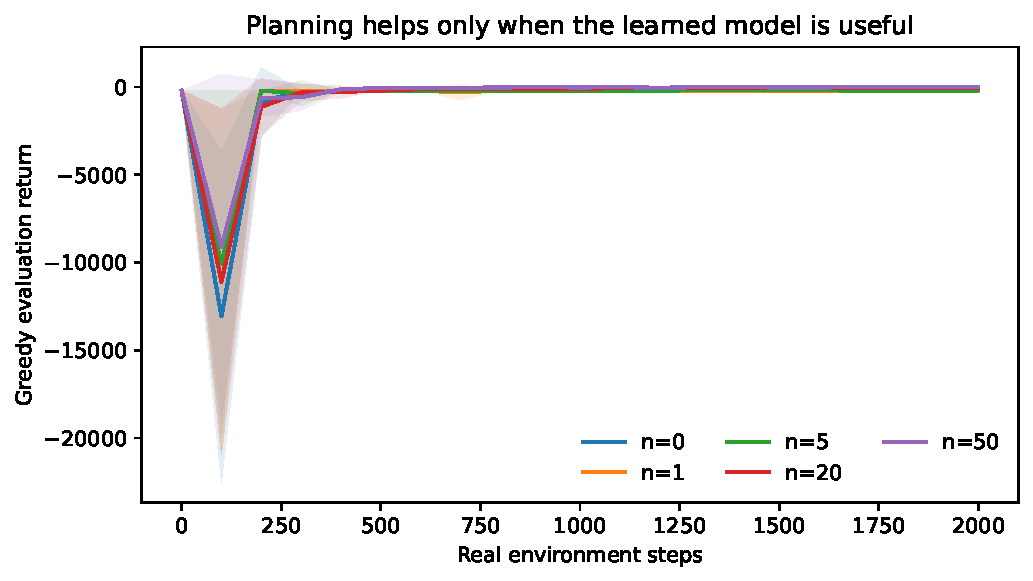
\includegraphics[width=0.88\textwidth]{fig1_sample_efficiency.pdf}
  \caption{CliffWalking-v0 上不同规划预算 $n$ 的固定真实步数评估曲线；均值与阴影由 20 个 seeds 的贪心评估得到。横轴是环境步数，不是 episode 编号，因此不同策略的 episode 长度不会改变比较基准。}
  \label{fig:dyna-sample-efficiency}
\end{figure}

% ============================================================
\section*{Dyna-Q 的核心机制}

\subsection*{真实更新与想象更新}

Dyna-Q 将两条路径放在同一个循环中。真实更新使用环境刚刚返回的转移，因此它同时修正模型和 Q；想象更新从模型中抽取此前见过的状态—动作对，只修正 Q。

\[
\boxed{
\begin{aligned}
\delta_{\mathrm{real}}&=r+\gamma(1-d)\max_{a'}Q(s',a')-Q(s,a),\\
\delta_{\mathrm{plan}}&=\hat r+\gamma(1-\hat d)\max_{a'}Q(\hat s',a')-Q(\hat s,\hat a).
\end{aligned}}
\]

两者使用相同的 Q 更新形式，但信息来源不同。真实更新承担纠错作用，规划更新承担传播作用；如果模型有系统偏差，规划也会系统性地放大该偏差。

\subsection*{规划次数 $n$ 的含义}

每完成一次环境步，先完成真实更新，再从 $\mathcal K$ 中随机抽取 $n$ 个状态—动作对。$n$ 越大，单位真实交互带来的计算量越大；当模型准确时，这通常带来更快的学习，当模型陈旧或错误时，则可能产生过度自信。

\begin{figure}[!htbp]
  \centering
  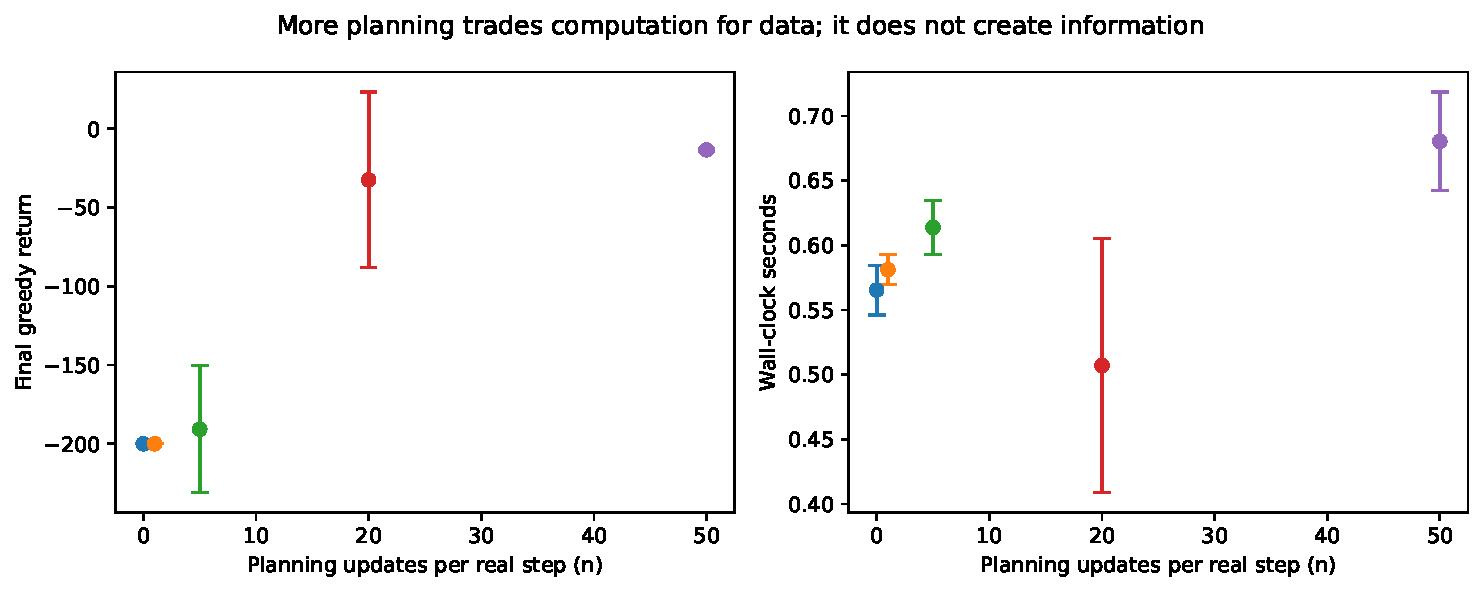
\includegraphics[width=0.88\textwidth]{fig2_planning_sweep.pdf}
  \caption{相同 2000 个真实环境步数后的最终贪心回报与墙钟时间；每个 $n$ 使用 20 个 seeds。左图衡量数据效率，右图显示规划计算的额外成本，不把模拟更新计作新样本。}
  \label{fig:dyna-planning-sweep}
\end{figure}

\subsection*{规划次数 $n$ 与规划深度不是一回事}

本章的 Dyna-Q 每次规划只做一个模型备份。$n$ 表示备份次数，不表示想象轨迹的深度：当模型中的奖励变化需要经过多个前驱状态传播时，必须让这些状态被反复抽到。另一种做法是从当前状态展开长度为 $H$ 的模型 rollout，构造

\[
\hat G_H=\sum_{j=0}^{H-1}\gamma^j\hat r_j+\gamma^H\max_a Q(\hat s_H,a).
\]

它并不等价于 $n=H$ 的 Dyna 更新：前者沿一条想象轨迹连续承受模型误差，后者把有限的备份分配到多个状态—动作对。$H$ 增大时，局部转移误差会通过多步组合累积；$n$ 增大时，主要改变的是计算分配。

\subsection*{优先级：为什么不应总是均匀采样}

均匀规划把每个已见状态—动作对视为同等重要，但奖励变化往往只影响一小片前驱区域。Prioritized Sweeping 为每个候选备份维护优先级

\[
p(s,a)=\left|\hat r+\gamma(1-\hat d)\max_{a'}Q(\hat s',a')-Q(s,a)\right|,
\]

每次取优先级最大的对更新，并把其模型前驱加入队列。这样，价值变化可以沿前驱图迅速向后传播；代价是维护前驱关系和队列，并且高优先级不等于高模型可信度。优先级解决的是\textbf{计算分配}，不是探索不确定性：$\epsilon$-greedy 决定去哪里收集真实数据，置信上界或不确定性 bonus 才是主动利用模型不确定性的另一类设计。


\subsection*{随机环境中的模型偏差：一个可复现的失败模式}

在 FrozenLake 这类随机环境中，同一个 $(s,a)$ 可能对应多个后继状态。只保存最后一次观测的确定性模型，会把随机性误读为确定性；保存经验频数则能表达不确定性，但在观测不足时仍然会有方差。规划的收益取决于模型误差、访问覆盖和规划预算三者的共同作用。

考虑一个两状态反例：动作 $a$ 以概率 $0.99$ 得到 $0$，以概率 $0.01$ 转移到奖励为 $+100$ 的状态。如果有限样本最后一次恰好是 $0$，last-observation 模型会低估动作；如果最后一次恰好是稀有的 $+100$，大量规划更新又会把一次偶然事件当成必然事件。$n$ 越大，错误模型被重复使用的次数越多。经验分布能随样本增加而收敛，但在覆盖不足时也不应被误读为真实核。这个反例说明：规划可以节省交互，却不能替代信息收集。
\begin{figure}[!htbp]
  \centering
  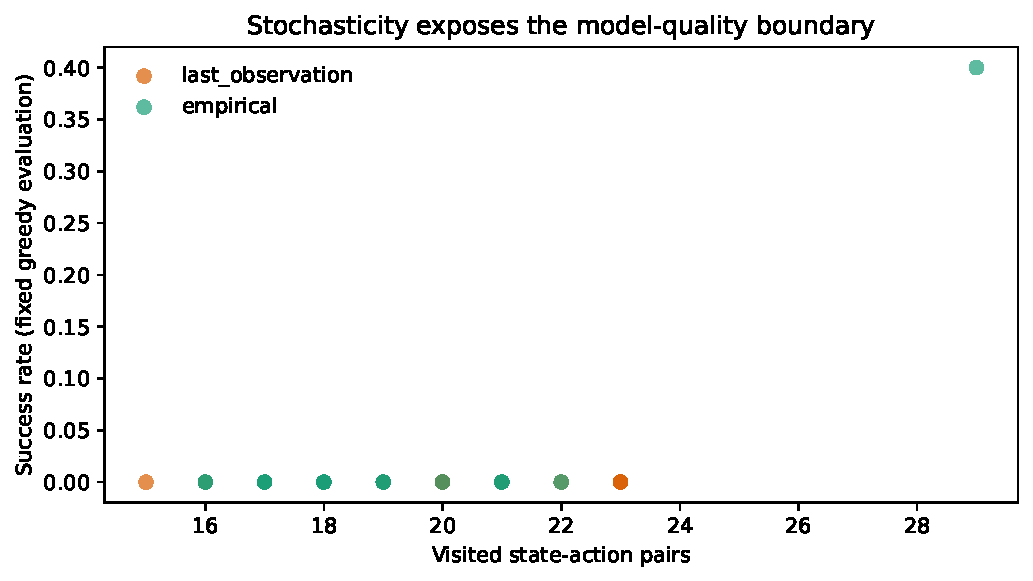
\includegraphics[width=0.88\textwidth]{fig3_model_bias.pdf}
  \caption{随机 FrozenLake-v1 中 last-observation 与 empirical 模型的覆盖—成功率诊断；每个点对应一个 seed，成功率来自固定、无探索的贪心评估。该图比较模型表示方式，不把相关性夸大为因果结论。}
  \label{fig:dyna-model-bias}
\end{figure}

在确定性 CliffWalking 上，模型一旦观察到 $(s,a)$ 的结果便可以精确复用；在随机 FrozenLake 上，模型还必须估计结果分布。为避免把两种误差混在一起，实验应分别报告：已见状态—动作覆盖率、模型预测的转移误差、真实环境步数、规划备份数，以及固定评估协议下的回报或成功率。图 3 的散点是诊断关系，而不是因果证明；它不能单独证明“不确定性导致回报下降”。


\subsection*{算法流程}

\begin{enumerate}
  \item \textbf{初始化}：$Q(s,a)=0$，模型为空，已见状态—动作集合 $\mathcal K=\varnothing$；
  \item \textbf{真实行动}：按 $\epsilon$-greedy 从当前 $Q$ 选择 $a$，与环境交互得到 $(s',r,d)$；
  \item \textbf{真实 Q 更新}：使用 $r+\gamma(1-d)\max_{a'}Q(s',a')$ 更新 $Q(s,a)$；
  \item \textbf{模型更新}：将 $(s',r,d)$ 写入 $\hat p(\cdot\mid s,a)$，并把 $(s,a)$ 加入 $\mathcal K$；
  \item \textbf{规划循环}：重复 $i=1,\ldots,n$，从 $\mathcal K$ 采样 $(\hat s,\hat a)$，从模型采样 $(\hat s',\hat r,\hat d)$，执行一次想象 Q 更新；
  \item \textbf{继续}：若环境终止则重置，否则令 $s\leftarrow s'$。
\end{enumerate}

这一顺序很重要：先把真实经验写入模型，再允许规划使用它。若先规划后更新模型，本次新信息就会被延迟一个循环。

\subsection*{与相邻方法对比}

\begin{itemize}
  \item \textbf{Q-learning}：$n=0$，只用真实转移更新价值；
  \item \textbf{Dyna-Q}：学习一个显式模型，并从模型中进行规划；
  \item \textbf{动态规划}：假设模型已知，直接对模型进行系统性备份；
  \item \textbf{模型预测控制}：通常在线滚动规划并执行短视动作序列，而不一定维护一个长期 Q 函数；
  \item \textbf{现代潜变量规划}：MuZero、Dreamer 等方法可以在学习到的潜空间中进行更复杂的 rollout，但同样面对模型偏差和分布覆盖问题。
\end{itemize}

% ============================================================
\section*{本章在 RL 体系中的位置}

\begin{enumerate}
  \item \textbf{上游}：MDP、TD learning 与 Q-learning 提供价值备份；
  \item \underline{\textbf{Dyna-Q}}：学习环境模型，并用真实经验与想象经验共同更新价值；
  \item \textbf{下游}：模型预测控制、潜变量世界模型、MuZero，以及带模型 rollout 的离线强化学习。
\end{enumerate}

本章最重要的结论是：模型式强化学习不是“无模型方法加一个预测器”这么简单，而是一个信息来源的分层系统。真实交互带来新信息，模型负责复用信息，规划负责传播信息；三者必须在实验中分开计量。下一步可以沿着模型误差与长时 rollout 的方向，学习更强的世界模型和不确定性估计。

\subsection*{参考资料}

\begin{enumerate}
  \item Sutton, R. S. (1991). Dyna, an integrated architecture for learning, planning, and reacting. \textit{ACM SIGART Bulletin}.
  \item Sutton \& Barto (2018). \textit{Reinforcement Learning: An Introduction} (2nd ed.). Chapter~9.
  \item Schrittwieser et al. (2020). Mastering Atari, Go, chess and shogi by planning with a learned model. \textit{Nature}.
\end{enumerate}

\end{document}
